% !TeX TS-program = txs:///latexmk | txs:///view-log | txs:///view-pdf | txs:///convert
\documentclass{article}
\usepackage{tikzducks}

\begin{document}


\begin{tikzpicture}
\duck
\end{tikzpicture}
\qquad
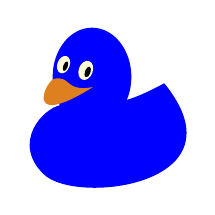
\begin{tikzpicture}
\duck[body=blue]
\end{tikzpicture}
\qquad

\begin{tikzpicture}
\duck[body=yellow,
			head=yellow!50!orange, 
			bill=red]
\end{tikzpicture}


\begin{tikzpicture}
\duck[longhair]
\end{tikzpicture}
\qquad

\begin{tikzpicture}
\duck[shorthair]
\end{tikzpicture}
\qquad

\begin{tikzpicture}
\duck[crazyhair]
\end{tikzpicture}


\begin{tikzpicture}
\duck[recedinghair]
\end{tikzpicture}
\qquad

\begin{tikzpicture}
\duck[longhair=teal]
\end{tikzpicture}
\qquad

\begin{tikzpicture}
\duck[grumpy]
\end{tikzpicture}


\begin{tikzpicture}
\duck[eyebrow]
\end{tikzpicture}
\qquad
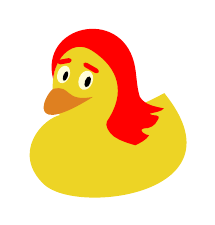
\begin{tikzpicture}
\duck[longhair=red, eyebrow]
\end{tikzpicture}
\qquad
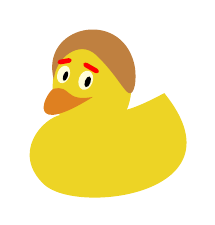
\begin{tikzpicture}
\duck[shorthair, eyebrow=red]
\end{tikzpicture}


\begin{tikzpicture}
\duck[water=cyan!50!blue]
\end{tikzpicture}
\qquad
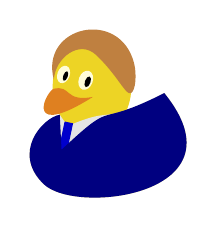
\begin{tikzpicture}
\duck[tshirt=white!80!gray, 
			jacket=blue!50!black, 
			tie=blue!80!black, 
			shorthair]
\end{tikzpicture}
\qquad

\begin{tikzpicture}
\duck[alien=green!50!brown]
\end{tikzpicture}


\begin{tikzpicture}
\duck[icecream]
\end{tikzpicture}
\qquad

\begin{tikzpicture}
\duck[icecream=brown, flavoura=brown, flavourb=white, flavourc=red]
\end{tikzpicture}
\qquad

\begin{tikzpicture}
\duck[hat=red!50!black]
\end{tikzpicture}


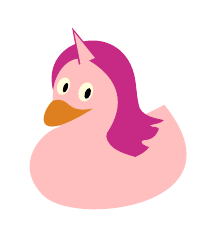
\begin{tikzpicture}
\duck[body=pink,
			unicorn=magenta!60!violet,
			longhair=magenta!60!violet]
\end{tikzpicture}
\qquad

\begin{tikzpicture}
\duck[glasses=red!50!black]
\end{tikzpicture}
\qquad

\begin{tikzpicture}
\duck[sunglasses]
\end{tikzpicture}

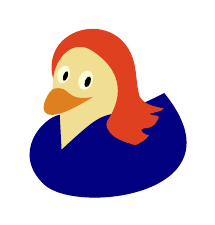
\begin{tikzpicture}
	\duck[body=yellow!50!brown!50!white, 
				longhair=red!50!brown, 
				jacket=blue!50!black]
\end{tikzpicture}
\qquad

\begin{tikzpicture}
	\definecolor{brazilgreen}{RGB}{0,155,58}
	\definecolor{brazilyellow}{RGB}{254,223,0}
	\definecolor{brazilblue}{RGB}{0,39,118}
	\duck[body=brazilyellow,
				jacket=brazilblue,
				shorthair=brazilgreen]
\end{tikzpicture}
\qquad

\begin{tikzpicture}
	\duck[grumpy,
				body=yellow!50!brown!50!white,
				tshirt=white,
				jacket=black,
				tie=black,
				hat=black,
				sunglasses=black]
\end{tikzpicture}

% prof. van duck

\begin{tikzpicture}
	\duck[body=yellow!50!brown!40!white,
				crazyhair=gray!50!white,
				eyebrow,
				glasses=brown!70!black,
				book=\scalebox{0.2}{$E=mc^2$},
				bookcolour=red!20!brown
]
\end{tikzpicture}
\qquad
% knuth
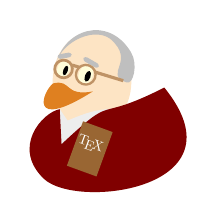
\begin{tikzpicture}
	\duck[body=yellow!50!red!20!white,
				recedinghair=gray!50!white,
				eyebrow,
				tshirt=white!93!black,
				jacket=red!50!black,
				glasses=brown!70!lightgray,
				book=\scalebox{0.5}{\TeX},
				bookcolour=black!20!brown
]
\end{tikzpicture}
\qquad

\begin{tikzpicture}
	\duck[magichat,
				magicwand]
\end{tikzpicture}



\begin{tikzpicture}
	\duck[magichat=teal,
				magicstars=cyan]
\end{tikzpicture}
\qquad
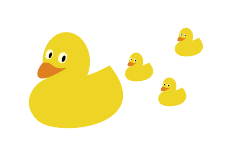
\begin{tikzpicture}[scale=0.6]
	\duck
	\begin{scope}[xshift=90pt, scale=.3, yshift=150pt]
		\duck
	\end{scope}
	\begin{scope}[xshift=60pt, scale=.3, yshift=100pt]
		\duck
	\end{scope}
	\begin{scope}[xshift=80pt, scale=.3, yshift=50pt]
		\duck
	\end{scope}		
\end{tikzpicture}


\end{document}
